
\section{Quantum-Classical Physics-Informed Neural Networks (QCPINN)} 
\label{sec:QCPINN}

\begin{figure}[t]
    \centering
    % 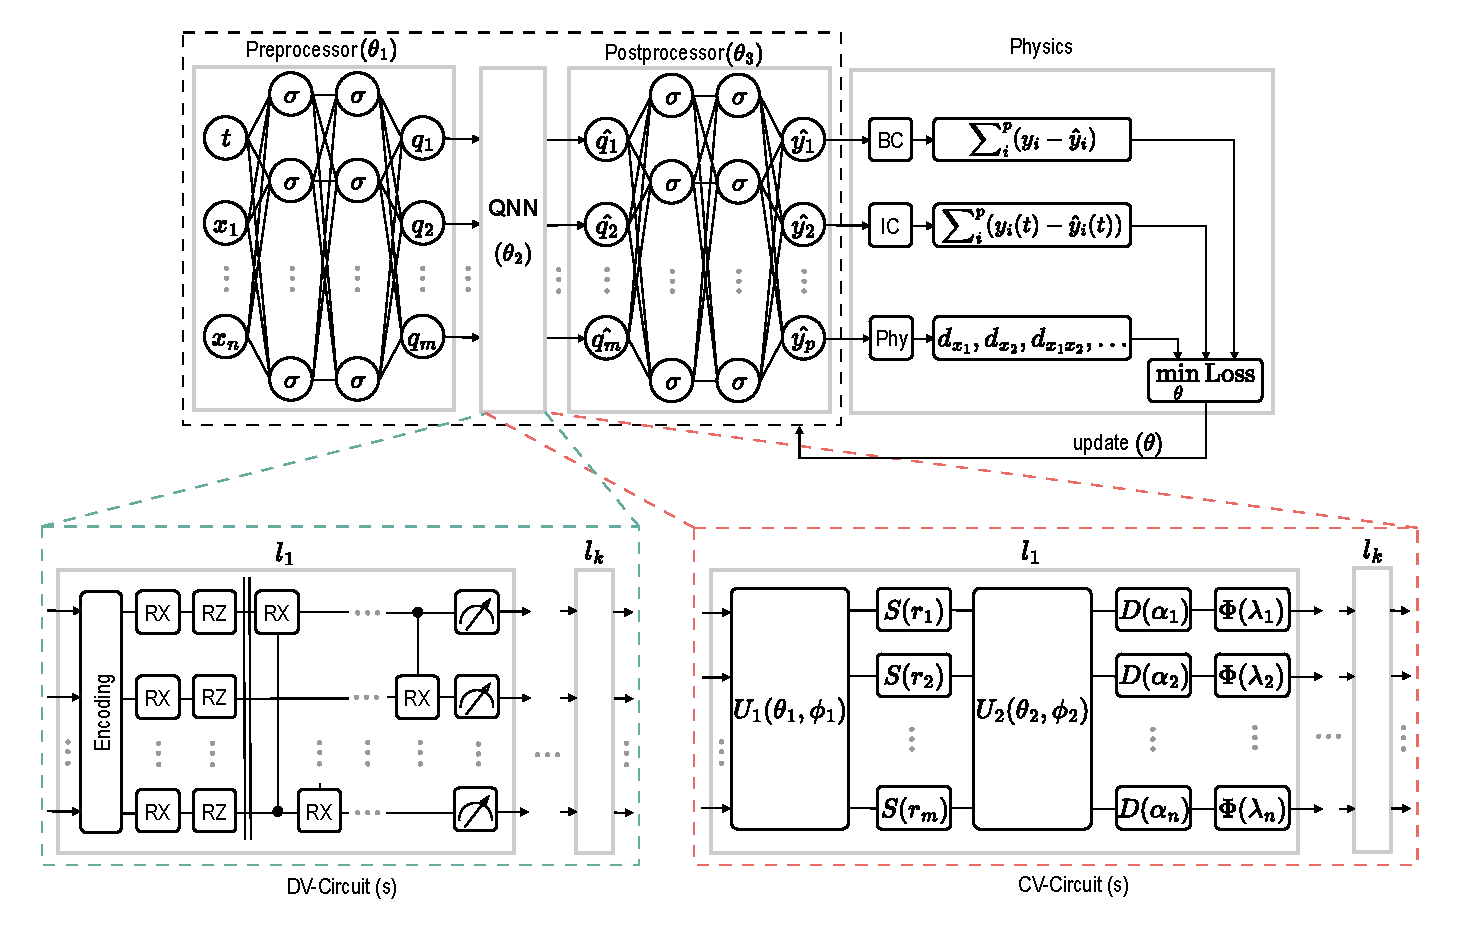
\includegraphics[width=0.9950\textwidth,trim=0.0cm 0.0cm 0.0cm 0.0cm, clip]{figures/QCPINN.pdf}    
    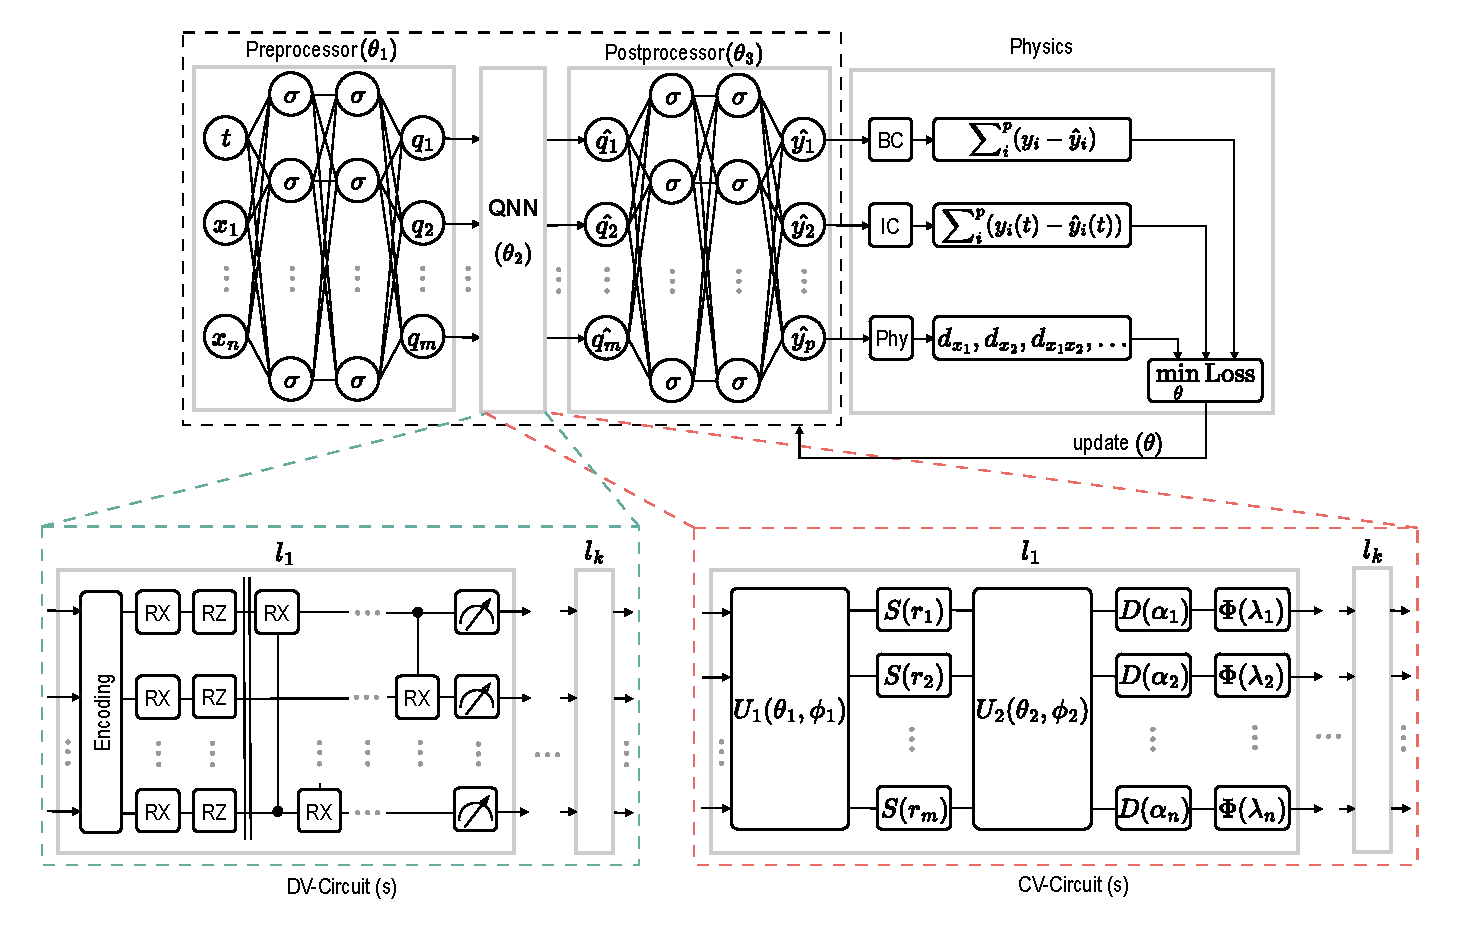
\includegraphics[width=0.99\textwidth,trim=0.0cm 0.0cm 0.0cm 0.0cm, clip]{figures/QCPINN.pdf}    
    \caption{Architecture of the quantum-classical physics-informed neural network (QCPINN) framework as introduced in section~\ref{sec:QCPINN}. The figure illustrates the hybrid structure: a classical preprocessor encodes the inputs, which are then fed into the quantum neural network, implemented as either CV-based or DV-based circuits with $k$ layers. A classical postprocessor then decodes the quantum outputs. The integrated loss function concurrently minimizes PDE residuals and initial/boundary condition errors, ensuring the model adheres to physical constraints throughout training.}
    \label{fig:architecture}
\end{figure}

\begin{figure}[t]
    \centering
    \begin{tabular}{cc}
        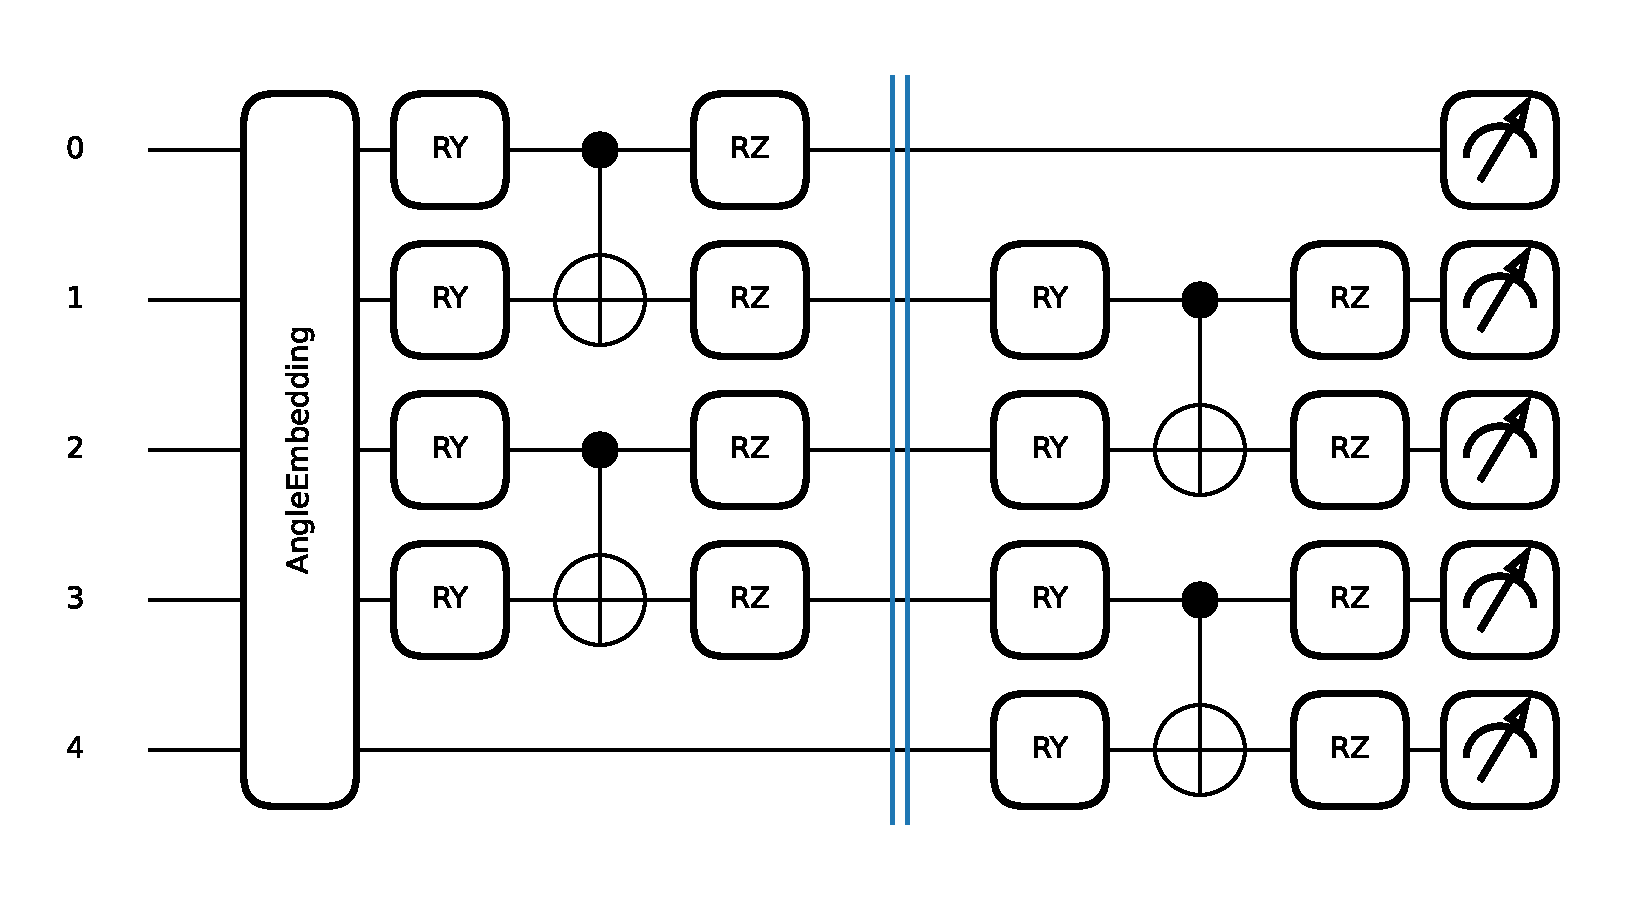
\includegraphics[width=0.40\columnwidth, trim={0.35cm 0.35cm 1.5cm 0.0cm}, clip]{figures/alternate.pdf} &
        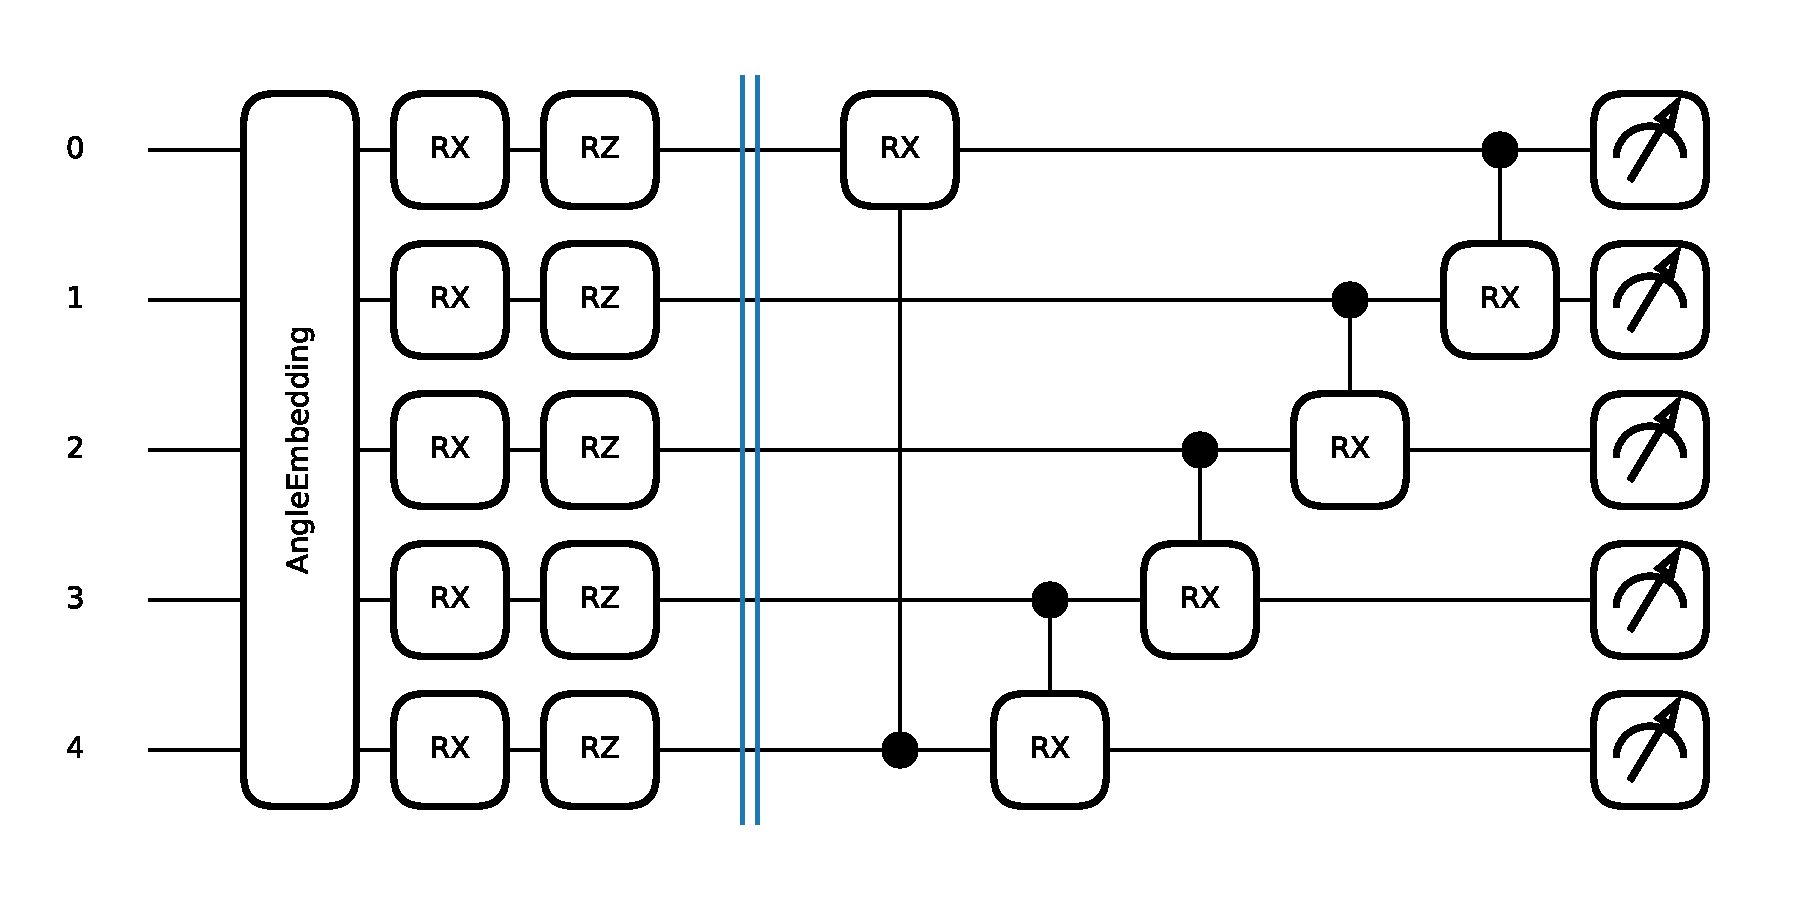
\includegraphics[width=0.45\columnwidth, trim={0.35cm 0.35cm 1.5cm 0.0cm}, clip]{figures/cascade.pdf} \\
        \footnotesize{(a) Alternate} & \footnotesize{(b) Cascade} \\
        \multicolumn{2}{c}{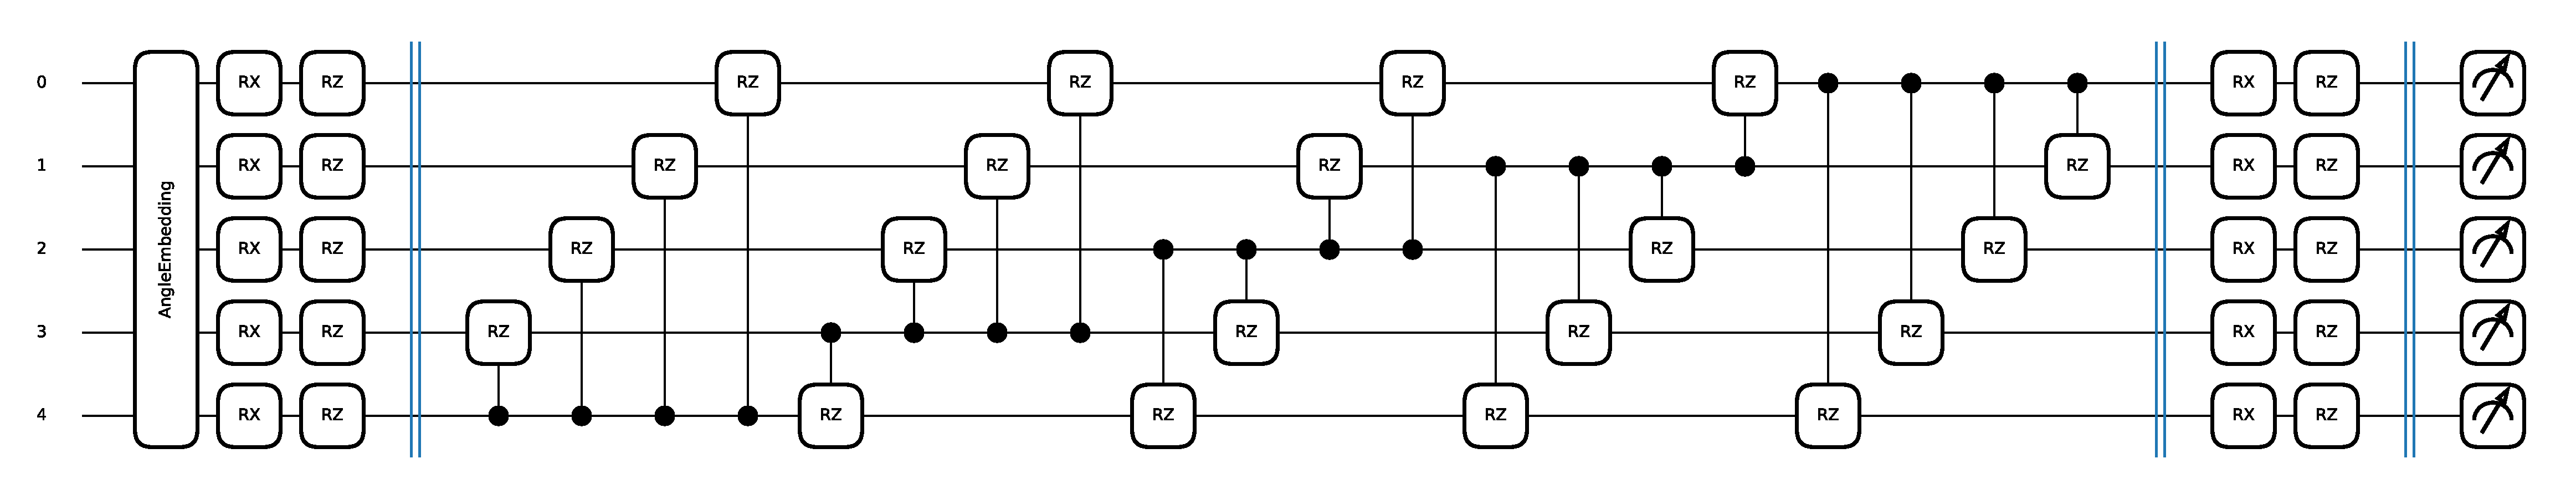
\includegraphics[width=0.97\columnwidth, trim={1.65cm 1.45cm 1.60cm 1.45cm}, clip]{figures/cross_mesh.pdf}} \\
        \multicolumn{2}{c}{\footnotesize{(c) Cross-mesh}} \\
        \multicolumn{2}{c}{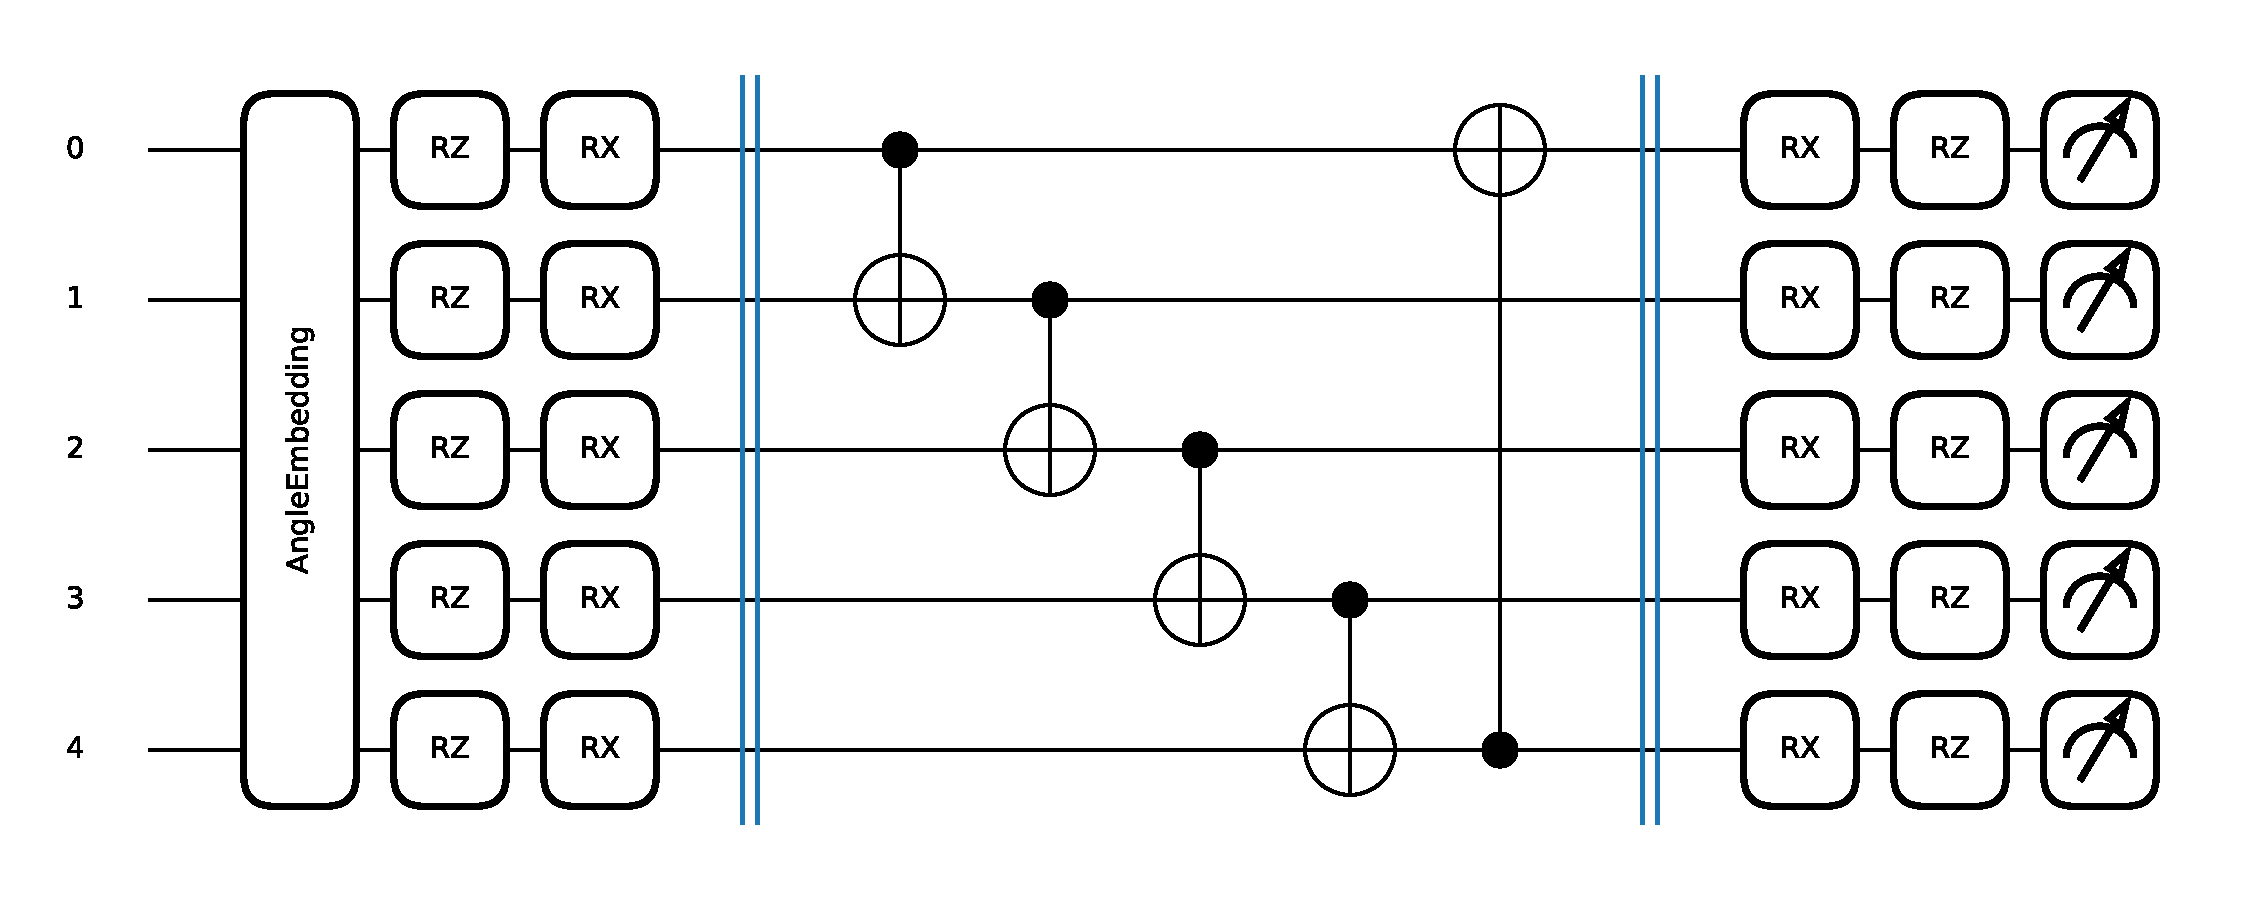
\includegraphics[width=0.65\columnwidth, trim={0.35cm 0.35cm 0.25cm 0.25cm}, clip]{figures/layered.pdf}} \\
        \multicolumn{2}{c}{\footnotesize{(d) Layered}}
    \end{tabular}
    \caption{Example PQC illustrated with angle encoding and five qubits. The rounded square gates represent parameterized rotation gates. The detailed characteristics of these circuits are provided in table~\ref{tab:circuit_comparison}.
    }
    \label{fig:dv_circuits}
\end{figure}


Figure~\ref{fig:architecture} provides a high-level overview of our proposed QCPINN. The preprocessing network comprises two classical layers, ensuring that the overall framework remains both shallow enough for efficient training and deep enough to capture essential transformations while maintaining differentiability throughout. Each layer consists of 50 neurons per layer with Tanh activation function. The first layer of the preprocessor performs a linear transformation that alters the input dimension, followed by a Tanh activation function to introduce non-linearity. The second layer then maps the transformed inputs to the quantum layers. Similarly, the postprocessing layer mirrors this structure with appropriate dimensions, ensuring a symmetric transformation between classical and quantum representations. This design provides flexibility in handling quantum feature representations while guaranteeing the higher-order differentiability required for residual loss in PINNs.

In the following subsections, we present two primary network architectures.  The first is the Continuous-Variable (CV-based) QCPINN, a hybrid model that leverages a photonic-based quantum neural network. The second is the Discrete-Variable (DV-based) QCPINN, which employs qubit-based quantum circuits. We introduce the Classical PINN, an entirely classical feedforward neural network trained within the PINN framework to validate these hybrid models. 

\subsection{CV-based QCPINN}

Following the proposed hybrid model in figure \ref{fig:architecture}, the architecture consists of three primary components: a classical preprocessing network, a quantum network, and a classical postprocessing network. The quantum network is implemented following the framework introduced in \cite{killoran2019continuous}, as outlined in algorithm \ref{alg:cv_qnn}. This network comprises multiple quantum layers, each executing a well-structured sequence of quantum operations. By structuring the network this way, the complete circuit depth scales as $(2n+3)L$, and the number of trainable quantum parameters grows as $\mathcal{O}(n^2 L)$, where  $n$ is the number of qumodes and $L$ is the number of layers. In contrast, classical feedforward neural networks follow a more flexible scaling pattern, with $\mathcal{O}(h^2 L)$ parameters, where $h$ represents the number of hidden neurons ( assuming a fixed width $h$ across all hidden layers). Besides, classical networks allow independent selection of $h$, providing greater architectural adaptability. Thus, while classical models rely on deep architectures and larger parameter counts, quantum networks achieve expressivity by leveraging intrinsic quantum correlations and physics-based constraints.

% \red{reference \ref{alg:cv_qnn}}

% \red{Initially we trained CV-based QPINN for testing Helmholtz and Cavity, see the results in~\ref{app:appendix_a}. However, the training convergence is not promising, therefore, we propose another approach called DV-based QCPINN and an extensive analysis of various approaches underpinning DV-based QCPINN in the following section.
% }

Initially, we trained the CV-based QCPINN to solve the Helmholtz and Cavity problems. However, the model exhibited severe convergence difficulties, with persistent fluctuations in the residual loss and an overall failure to effectively minimize the governing equation error. As shown in figure~\ref{fig:cv_loss_plots}, while the boundary condition loss gradually decreased, the physical loss remained high, suggesting that the model struggled to capture the underlying physics of the PDEs. This instability persisted despite extensive hyperparameter tuning, indicating intrinsic limitations in the CV-based formulation. In contrast, as discussed in the following section, the DV-based QCPINN demonstrated better training efficiency and stability, achieving significantly lower error rates and more reliable convergence across different PDE benchmarks.





\begin{table}[!t]
    \centering
    \caption{Comparison of different quantum circuit ansatz used in the study (as in figure~\ref{fig:dv_circuits}). $n$ is the number of qubits, and $L$ is the number of layers.}
    \label{tab:circuit_comparison}
    \scriptsize
    \begin{tabular}{l|c|c|c|c}
        \hline
        \textbf{Circuit} & \textbf{\makecell{Circuit \\Depth}} & \textbf{\makecell{Circuit \\Connectivity}} & \textbf{\makecell{Number of\\ Parameters}} & \textbf{\makecell{Number of\\ two-qubit gates}}  \\
        \hline
        (a) Alternate &  $6L$& Nearest-neighbor & $4(n-1)L$ & $(n-1)L$  \\
        (b) Cascade & $(n + 2)L$ & Ring topology & $3nL$ & $nL$  \\
        (c) Cross-mesh & $(n^2 - n + 4)L$ & All-to-all & $(n^2 +3n)L$  & $(n^2 -n)L$  \\
        (d) Layered &  $6L$& Nearest-neighbor & $4(n-1)L$ & $ (n-1)L$  \\
        \hline
    \end{tabular}
\end{table}

\subsection{DV-based QCPINN}

As shown in figure~\ref{fig:architecture}, the architecture comprises three main components: a classical preprocessing network, a quantum network, and a classical postprocessing network. The quantum network employs a custom DVQuantumNetwork, which executes quantum operations on the preprocessed data. Figure (\ref{fig:dv_circuits}) presents an example of four proposed PQC ansätze named after their architecture: Layered, Cross-mesh, Cascade, and Alternate. These circuits are inspired by the literature~\cite{farhi2018classification,sim2019expressibility,jaderberg2020minimum,setty2023physics}. Table~(\ref{tab:circuit_comparison}) compares these parameterized quantum circuits across key descriptors, including circuit depth, connectivity, number of parameters, and the number of two-qubit gates. 


According to Equation~(10) in~\cite{mouton2024deep}, a hardware-efficient ansatz (HEA) is defined as
\begin{equation}
\label{eq:HEA}
U(\theta) \;=\; \prod_{k} U_k(\theta_k) \, W_k,
\end{equation}
where each layer $k$ alternates between single-qubit parameterized rotations, $U_k(\theta_k)$, and an entangling operation, $W_k$. All four circuits in figure~\ref{fig:dv_circuits} adhere to this HEA structure. The selected circuit ansätze also agree with the affine transformation discussed in section~\ref{sec:background}.

Table~\ref{tab:circuit_comparison} compares these parameterized quantum circuits across key descriptors, including circuit depth, connectivity, number of parameters, and the number of two-qubit gates.

The \textit{Cross-mesh} ansatz demonstrates the highest expressibility among the evaluated circuits due to its quadratic scaling in the number of parameters. The circuit implements an all-to-all connectivity scheme, facilitating extensive interaction between qubits, which improves its capacity to explore the Hilbert space. The circuit depth scales as $(n^2 - n + 4)L$, while the count of trainable parameters is $(n^2 + 3n)L$. The utilization of global entanglement fosters strong correlations between qubits; however, this incurs larger circuit depth, resource demands, and difficulty of training~\cite{holmes2022connecting}. The total number of two-qubit gates in this circuit is $(n^2 - n)L$, which is considerably higher than other ansätze.

The \textit{Cascade} ansatz balances expressibility and hardware efficiency by employing a ring topology for qubit connectivity. This design facilitates efficient entanglement while keeping the circuit depth manageable at $(n+2)L$. The circuit contains $3nL$ trainable parameters, making it more efficient than Cross-mesh while preserving reasonable expressibility. Incorporating controlled rotation gates (CRX) enhances entanglement compared to CNOT gates and increases the circuit's capacity to explore the Hilbert space. Furthermore, the requirement for two-qubit gates is $nL$, which is fewer than that of Cross-mesh, thus lowering the overall computational cost.

The \textit{Layered} ansatz features a structured design comprising alternating rotation and entangling layers. Each qubit experiences parameterized single-qubit rotations, typically utilizing $R_X$ and $R_Z$ gates, introducing trainable parameters into the circuit. Entanglement is realized through nearest-neighbor CNOT gates, ensuring compatibility with hardware constraints while maintaining efficient connectivity. The circuit depth scales as $6L$, with a total of $4(n-1)L$ trainable parameters and $(n-1)L$ two-qubit gates, creating a balanced approach in terms of expressibility and hardware efficiency. Compared to Cross-mesh's all-to-all connectivity or Cascade's ring topology, the layered architecture represents a compromise between expressivity and hardware efficiency. 

The \textit{Alternate} ansatz employs an alternating-layer structure with nearest-neighbour CNOT gates, ensuring good entanglement while maintaining a manageable circuit depth of $6L$. This design leverages the repeated application of parameterized single-qubit rotations and CNOT layers to enhance expressibility. The number of trainable parameters in this circuit is $4(n-1)L$, which aligns with the Layered ansatz. The entanglement structure, dictated by the alternating CNOT layers, provides the highest level of entangling capability among the circuits studied. Furthermore, the number of two-qubit gates is $(n-1)L$, making it comparable to the Layered circuit in terms of hardware feasibility while achieving better entanglement. This renders the Alternate ansatz particularly advantageous for applications requiring high levels of entanglement with a controlled parameter count.
%
Hence, the Cross-mesh ansatz provides the largest parameter count and highest expressivity, while the Alternate circuit excels in entangling capabilities.

